\documentclass[12pt,letterpaper]{exam}
\usepackage[lmargin=1in,rmargin=1in,tmargin=1in,bmargin=1in]{geometry}
\usepackage{../style/exams}

% -------------------
% Course & Exam Information
% -------------------
\newcommand{\course}{MAT 101: Exam 2}
\newcommand{\term}{Spring -- 2022}
\newcommand{\examdate}{04/14/2022}
\newcommand{\timelimit}{85 Minutes}

\setbool{hideans}{true} % Student: True; Instructor: False

% -------------------
% Content
% -------------------
\begin{document}

\examtitle
\instructions{Write your name on the appropriate line on the exam cover sheet. This exam contains \numpages\ pages (including this cover page) and \numquestions\ questions. Check that you have every page of the exam. Answer the questions in the spaces provided on the question sheets. Be sure to answer every part of each question and show all your work.} 
\scores
%\bottomline
\newpage

% ---------
% Questions
% ---------
\begin{questions}

% Question 1
\newpage
\question[10] Sketch the quadratic function $f(x)= 8 - \left( x - \dfrac{13}{2} \right)^2$ on the plot below. Your sketch should include the vertex and axis of symmetry---being placed as accurately as possible. 
	\[
	\fbox{
	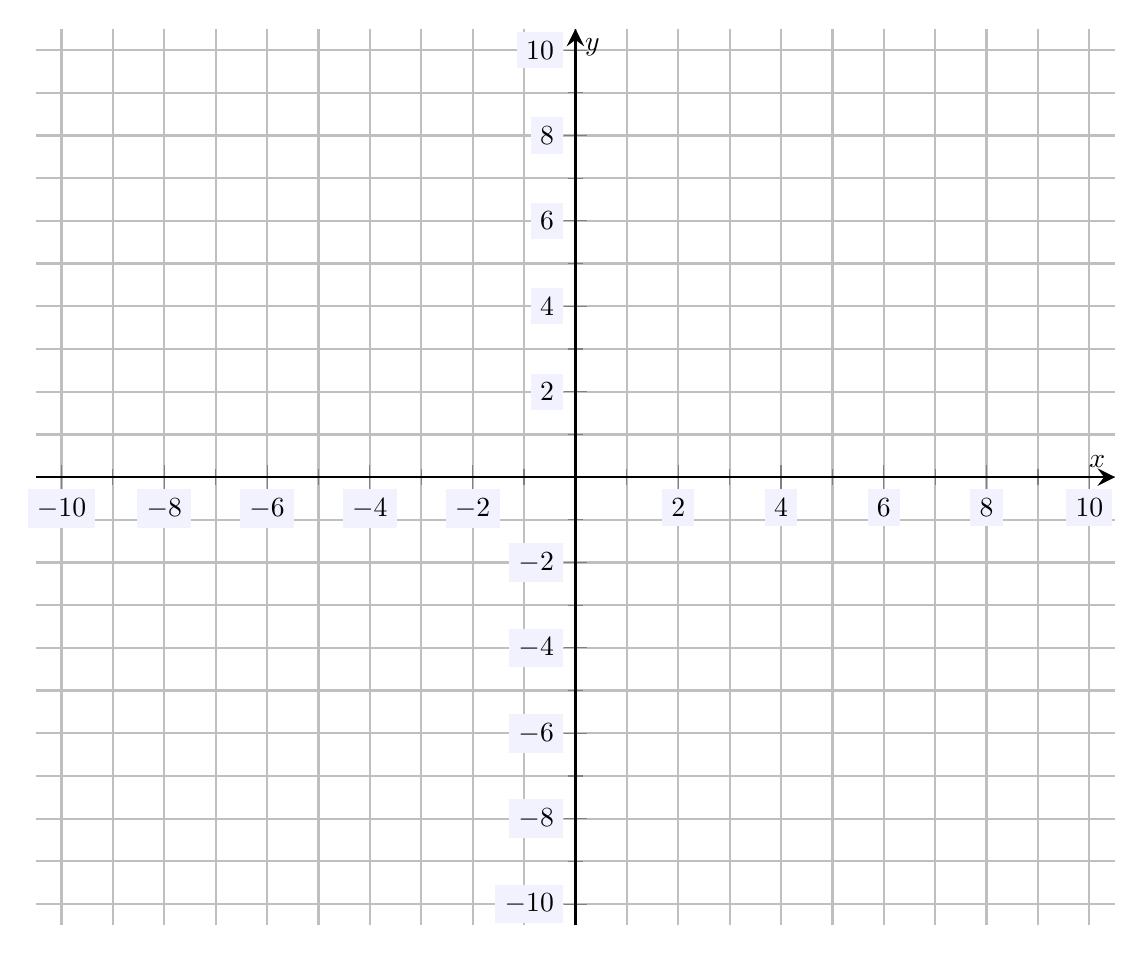
\begin{tikzpicture}[scale=2,every node/.style={scale=0.5}]
	\begin{axis}[
	grid=both,
	axis lines=middle,
	ticklabel style={fill=blue!5!white},
	xmin= -10.5, xmax=10.5,
	ymin= -10.5, ymax=10.5,
	xtick={-10,-8,-6,-4,-2,0,2,4,6,8,10},
	ytick={-10,-8,-6,-4,-2,0,2,4,6,8,10},
	minor tick = {-10,-9,...,10},
	xlabel=\(x\),ylabel=\(y\),
	]
	\end{axis}
	\end{tikzpicture}
	}
	\]



% Question 2
\newpage
\question Consider the quadratic function $y= (x + 5)^2 + 6$.

\begin{parts}
\part[2] Identify $a$, $b$, and $c$ for this quadratic function. \vfill
\part[2] Does this quadratic function open upwards or downwards? \vfill
\part[2] Is this quadratic function convex or concave? \vfill
\part[2] What is the vertex of this quadratic function? What is the axis of symmetry? \vfill
\part[2] Find the maximum and minimum values for $y$. \vfill
\end{parts}



% Question 3
\newpage
\question[10] Find the vertex form of the quadratic function $f(x)= -3x^2 + 12x - 7$. 



% Question 4
\newpage
\question[10] Factor $x^2 + 16x - 80$ completely. 



% Question 5
\newpage
\question[10] Factor $3x^2 - 9x - 120$ completely. 



% Question 6
\newpage
\question Factor the following completely: \pspace

\begin{parts}
\part[5] $16x - 20x^2$ \vfill
\part[5] $49 - x^2$ \vfill
\end{parts}



% Question 7
\newpage
\question[10] Factor $10x^2 + 43x - 35$ completely. 



% Question 8
\newpage
\question[10] Solve the following:
	\[
	5(6 - x)= \dfrac{4}{3}\,x + 30
	\]



% Question 9
\newpage
\question[10] Solve the following:
	\[
	9= x(10 - x)
	\]



% Question 10
\newpage
\question[10] Solve the following:
	\[
	6 - x= 12x + 7
	\]



% Question 11
\newpage
\question[10] Solve the following:
	\[
	x(3x - 1)= x(x + 5)
	\]



% Question 12
\newpage
\question[10] Solve the following:
	\[
	5(x + 5)= 4x^2 + 5x
	\]



% Question 13
\newpage
\question[10] Use the quadratic formula to solve the following:
	\[
	6 - 5x^2= 4x(1 - x)
	\]



% Question 14
\newpage
\question[10] Use the quadratic formula to factor $x^2 - 10x + 23$. 



% Question 15
\newpage
\question[10] Use the discriminant to determine whether the function $384x^2 + 232x - 175$ factors `nicely', i.e. over the integers. If not, determine whether it even factors over the real numbers or requires complex numbers to factor. 



% Question 16
\newpage
\question[10] Showing all your work, determine if the point $(5, -4)$ is a solution to the following system of equations:
	\[
	\begin{aligned}
	2x + y&= 6 \\[0.3cm]
	-5x - 6y&= -49
	\end{aligned}
	\]



% Question 17
\newpage
\question[10] Showing all your work, determine whether the following system of equations has a solution. If it has a solution, you do not need to find the solution.
	\[
	\begin{aligned}
	10x - 4y&= -24 \\[0.3cm]
	-5x + 2y&= -2
	\end{aligned}
	\]



% Question 18
\newpage
\question[10] Solve the following system of equations:
	\[
	\begin{aligned}
	3x + 5y&= 16 \\[0.3cm]
	x + 6y&= 1
	\end{aligned}
	\]



% Question 19
\newpage
\question[10] Solve the following system of equations:
	\[
	\begin{aligned}
	4x + 7y&= -8 \\[0.3cm]
	2x - 5y&= -4
	\end{aligned}
	\]



% Question 20
\newpage
\question[10] A quadratic function $y= x^2 - 2x + 1$ and a linear function $y= x + 1$ are plotted below.
	\[
	\fbox{
	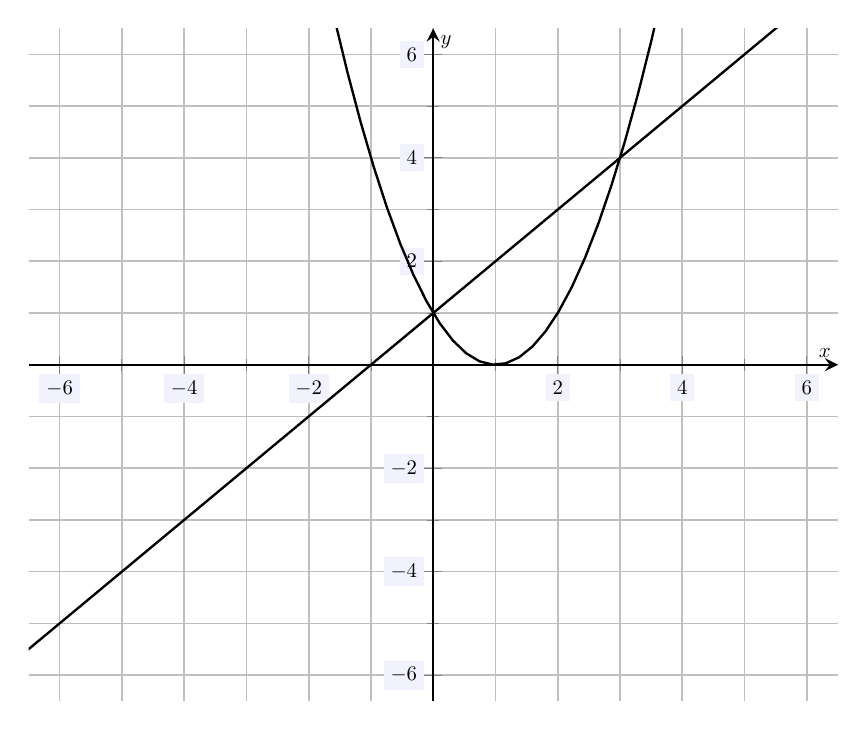
\begin{tikzpicture}[scale=1.5,every node/.style={scale=0.5}]
	\begin{axis}[
	grid=both,
	axis lines=middle,
	ticklabel style={fill=blue!5!white},
	xmin= -6.5, xmax=6.5,
	ymin= -6.5, ymax=6.5,
	xtick={-6,-4,-2,0,2,4,6},
	ytick={-6,-4,-2,0,2,4,6},
	minor tick = {-7,-6,...,7},
	xlabel=\(x\),ylabel=\(y\),
	]
	\addplot[line width= 0.02cm,samples=100,domain= -10.5:10.5] ({x},{x^2 - 2*x + 1}); 
	\addplot[line width= 0.02cm,samples=100,domain= -10.5:10.5] ({x},{x + 1}); 
	\end{axis}
	\end{tikzpicture}
	}
	\] \pspace

\begin{parts}
\part[5] Using the plot above, solve the following system of equations:
	\[
	\begin{aligned}
	-x + y&= 1 \\
	2x + y&= x^2 + 1
	\end{aligned}
	\] \pvspace{3cm}

\part[5] Setting the functions equal, verify the solution(s) to the system of equations from (a).
\end{parts}


\end{questions}
\end{document}